\documentclass[xcolor=svgnames]{beamer}
\usepackage[utf8]{inputenc}
\usepackage[english]{babel}

\newcommand{\semitransp}[2][35]{\color{fg!#1}#2}
\usepackage{wrapfig}

\usetheme{Proso}

\title[slepemapy.cz]{Rozšíření funkcionality slepemapy.cz}
\author{Vít Stanislav}
\institute{Fakulta informatiky Masarykovy univerzity}      % Enter your institute name between curly braces
\date{10. 12. 2014}

\begin{document}
% --------------------------- SLIDE --------------------------------------------
\frame[plain]{\titlepage}
% ------------------------------------------------------------------------------
% --------------------------- SLIDE --------------------------------------------
\begin{frame}
	\frametitle{Obsah}
  \begin{itemize}
  \huge \item slepemapy.cz před projektem
  \huge \item implementovaná rozšíření
  \huge \item současný stav aplikace
  \end{itemize}
\end{frame}
% ------------------------------------------------------------------------------
% --------------------------- SLIDE --------------------------------------------
\begin{frame}
	\frametitle{Obsah}
  \begin{itemize}
  \huge \item slepemapy.cz před projektem
  \semitransp[20]{ \huge \item implementovaná rozšíření
  \huge \item současný stav aplikace}
  \end{itemize}
\end{frame}
% ------------------------------------------------------------------------------
% --------------------------- SLIDE --------------------------------------------
\begin{frame}
	\frametitle{Procvičování států}
   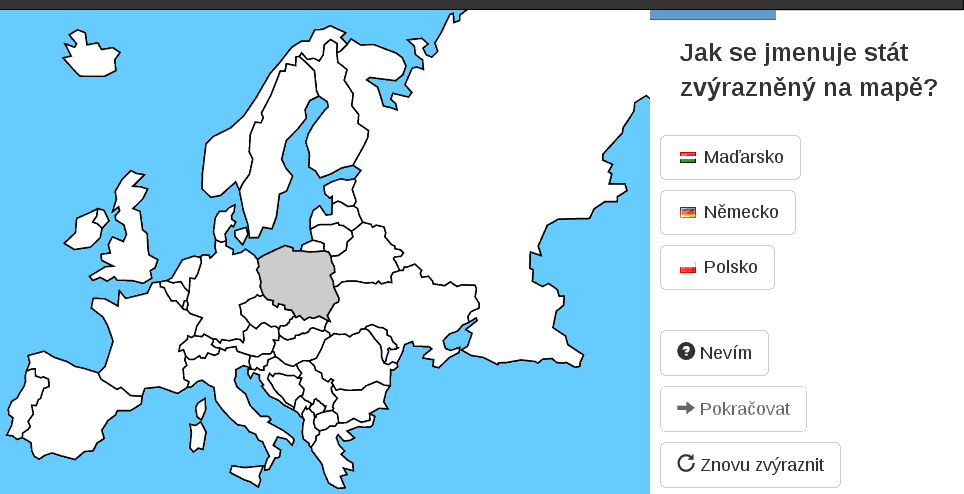
\includegraphics[width=\textwidth]{img/practice-example-cs.png}
\end{frame}
% ------------------------------------------------------------------------------
% --------------------------- SLIDE --------------------------------------------
\begin{frame}
	\frametitle{Výběr vhodných otázek}
  \begin{columns}
   \begin{column}{.49\textwidth}
      Odhad parametrů z odpovědí uživatelů 
      \begin{itemize}
        \item obtížnost státu
        \item celková znalost uživatele
        \item znalost daného státu 
      \end{itemize}
      Kritéria výběru otázky 
      \begin{itemize}
        \item přiměřená obtížnost 
        \item neopakovat stejný stát hned
        \item učení všech států na mapě 
      \end{itemize}
    \end{column}
    \begin{column}{.49\textwidth}
       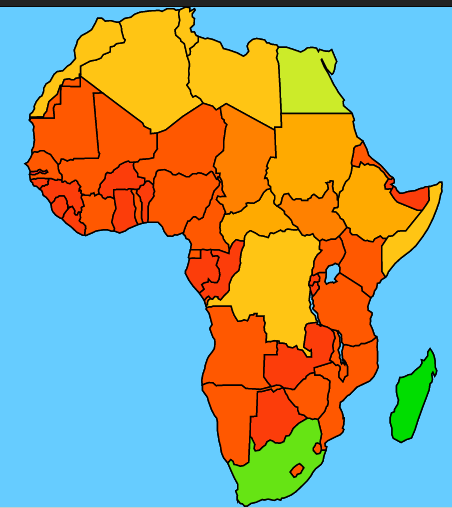
\includegraphics[width=\textwidth]{img/knowledge-map.png}
    \end{column}
  \end{columns}
\end{frame}
% ------------------------------------------------------------------------------
% --------------------------- SLIDE --------------------------------------------
\begin{frame}
	\frametitle{Obsah}
  \begin{itemize}
  \semitransp[20]{\huge \item slepemapy.cz před projektem}
  \semitransp[100]{ 
  \huge \item implementovaná rozšíření
  }
  \semitransp[20]{\huge \item současný stav aplikace}
  \end{itemize}
\end{frame}
% ------------------------------------------------------------------------------
% --------------------------- SLIDE --------------------------------------------
\begin{frame}
	\frametitle{Podpora pro města, řeky, jezera, ...}
   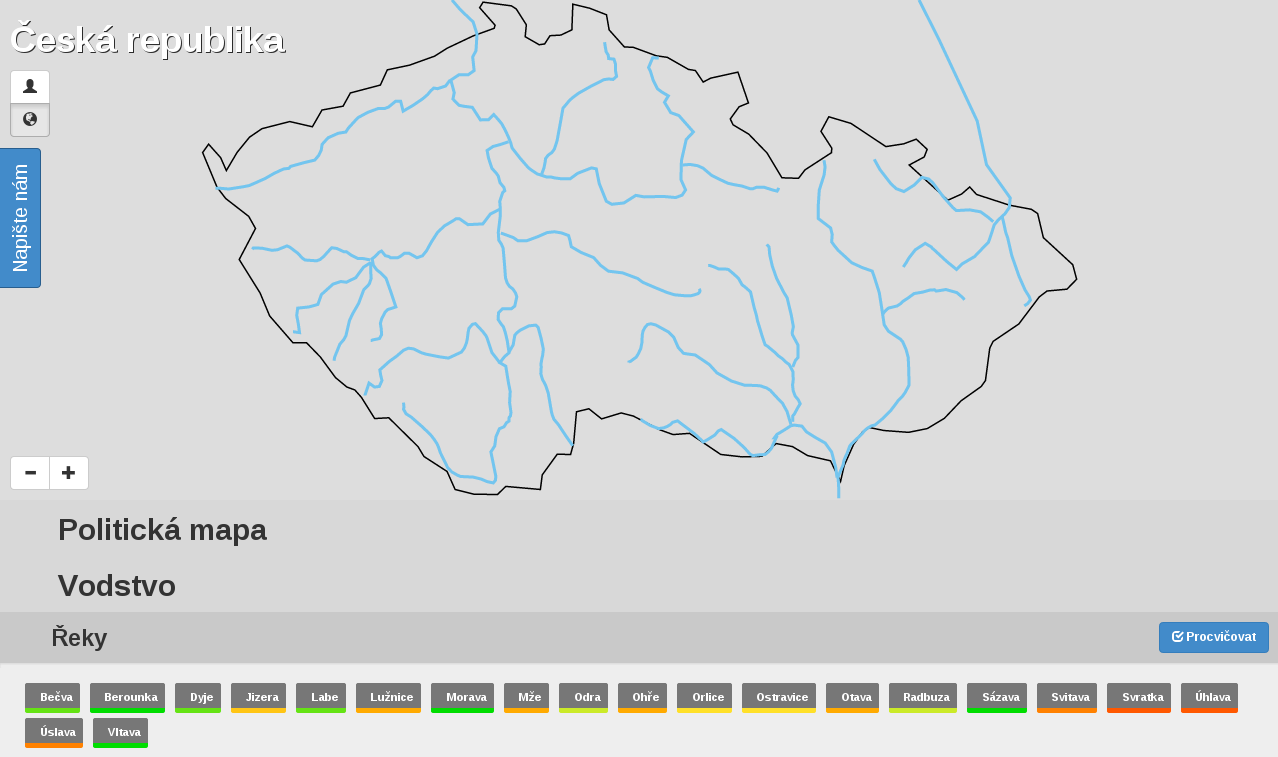
\includegraphics[width=\textwidth]{img/map-rivers.png}
\end{frame}
% ------------------------------------------------------------------------------
% --------------------------- SLIDE --------------------------------------------
\begin{frame}
	\frametitle{Optimalizace pro vyhledávače (SEO)}
   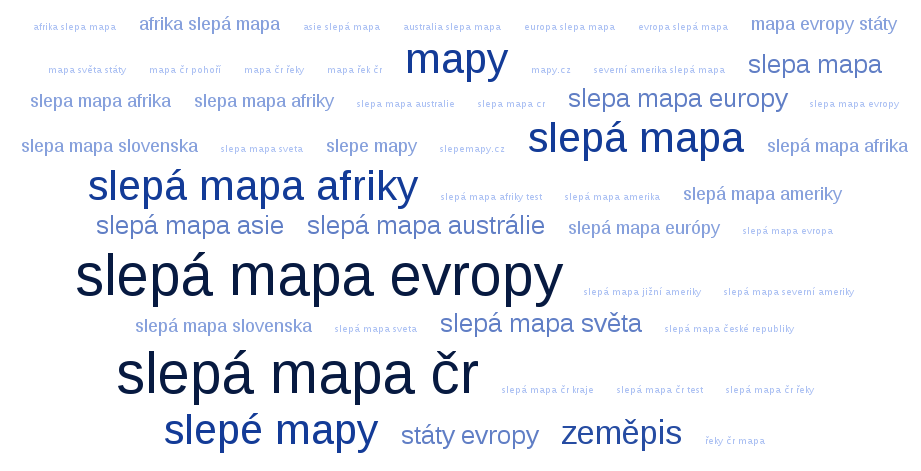
\includegraphics[width=\textwidth]{img/keywords-cloud.png}
\end{frame}
% ------------------------------------------------------------------------------
% --------------------------- SLIDE --------------------------------------------
\begin{frame}
	\frametitle{Přehled map}
   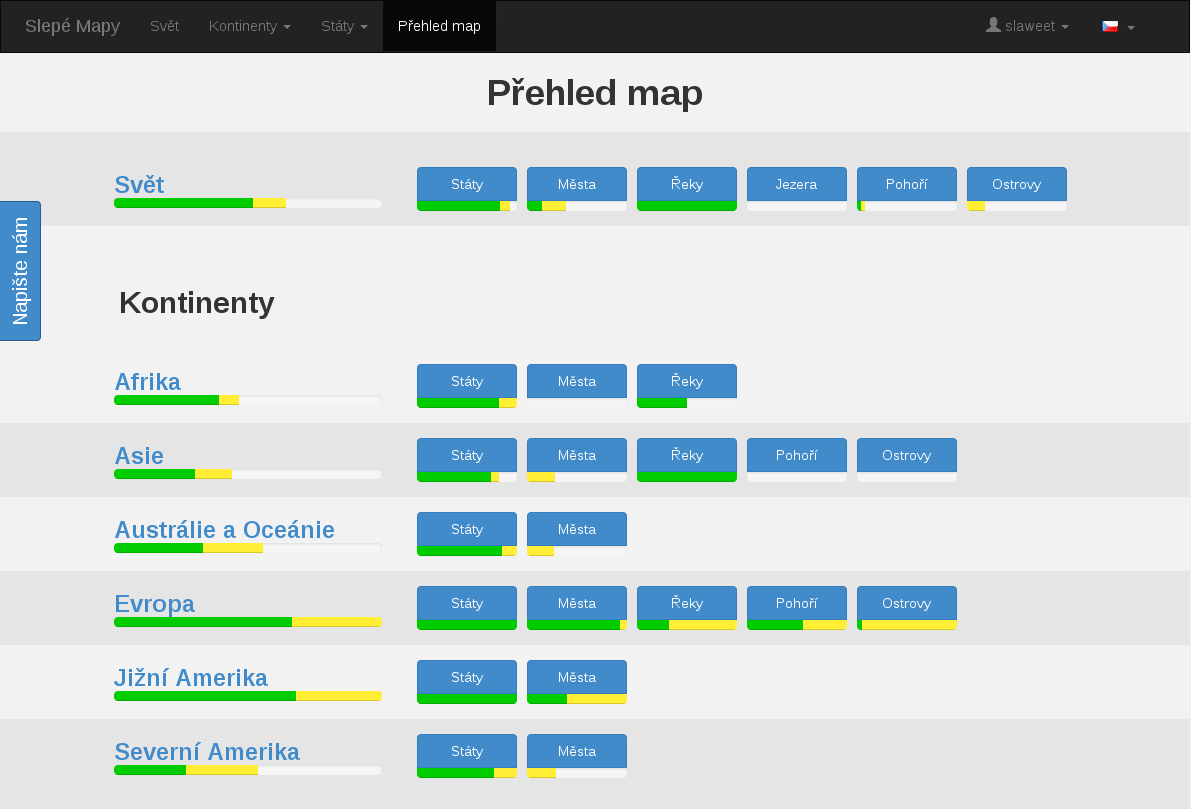
\includegraphics[width=\textwidth]{img/overview.png}
\end{frame}
% ------------------------------------------------------------------------------
% --------------------------- SLIDE --------------------------------------------
\begin{frame}
  \frametitle{Mnoho dalších vylepšení a oprav chyb}
  \begin{itemize}
  \item přiblížení mapy
  \item optimalizace vykreslování mapy
  \item optimalizace SQL dotazu pro mapu znalostí
  \item progress bar procvičených a naučených států na mapě znalostí
  \item automatizace nasazení front-endu pomocí Grunt
  \item přepracování hlavní strany – přímé odkazy na procvičování vybraných map
  \item tlačítka pro sdílení na sociálních sítích
  \end{itemize}
   Celkem  266 Git commitů.
\end{frame}
% ------------------------------------------------------------------------------
% --------------------------- SLIDE --------------------------------------------
\begin{frame}
	\frametitle{Obsah}
  \begin{itemize}
  \semitransp[20]{ 
    \huge \item slepemapy.cz před projektem
    \huge \item implementovaná rozšíření
  }
  \semitransp[100]{ 
  \huge \item současný stav aplikace
  }
  \end{itemize}
\end{frame}
% ------------------------------------------------------------------------------
% --------------------------- SLIDE --------------------------------------------
\begin{frame}
	\frametitle{Provoz aplikace}
	 Návštěvnost listopad 2013 - listopad 2014
   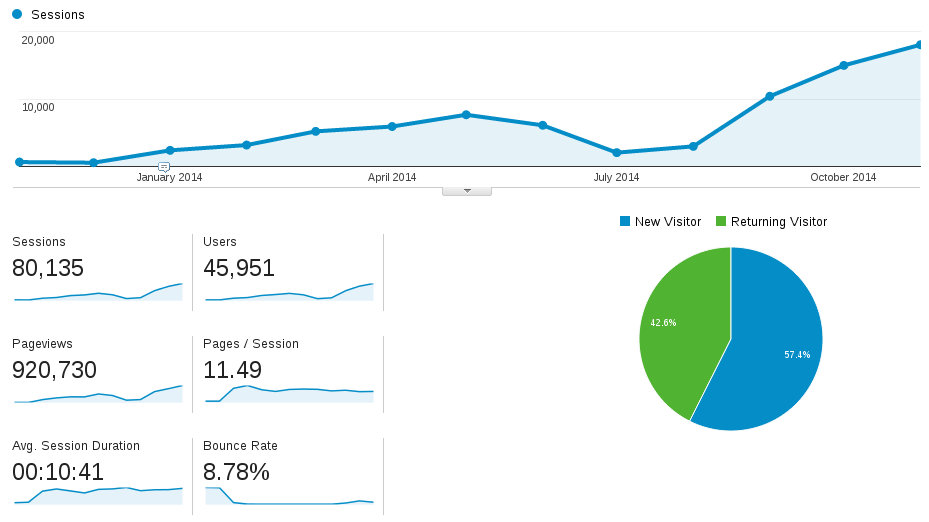
\includegraphics[width=\textwidth]{img/audience.png}
\end{frame}
% ------------------------------------------------------------------------------
% --------------------------- SLIDE --------------------------------------------
\begin{frame}
	\frametitle{Provoz aplikace}
	 Návštěvnost listopad 2014
   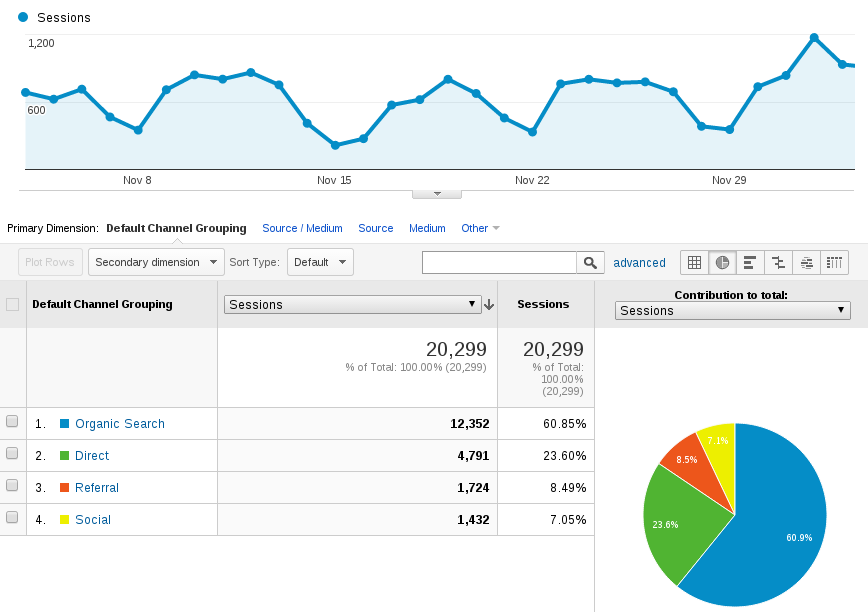
\includegraphics[width=\textwidth]{img/audience-latest.png}
\end{frame}
% ------------------------------------------------------------------------------
% --------------------------- SLIDE --------------------------------------------
\begin{frame}
	\frametitle{Další využití}
  \begin{itemize}
  \item Adaptive Practice of Facts in Domains with Varied Prior Knowledge (EDM 2014)
  \item Adaptive Learning Group - experimenty s posbíranými daty
  \item Dionýz Lazar - Analýza dat ze systému pro výuku zeměpisu (bakalářská práce)
  \item Jan Kučera - Adaptabilní webový systém pro výuku anatomie, slepaanatomie.cz (diplomová práce)
  \end{itemize}
\end{frame}
% ------------------------------------------------------------------------------
% --------------------------- SLIDE --------------------------------------------
\begin{frame}
  \frametitle{Konec}
\begin{center} 
\huge  Díky za pozornost.
\end{center}
\end{frame}
% ------------------------------------------------------------------------------
\end{document}
